\documentclass[oneside]{memoir}
\usepackage{fontspec}
\usepackage[hidelinks]{hyperref}
\usepackage{microtype}
\usepackage{amsmath}
\usepackage{amssymb}
\usepackage{bm}
\usepackage{xcolor}
\usepackage{booktabs}
\usepackage{graphicx}
\usepackage[euler-digits,euler-hat-accent]{eulervm}

\setlrmarginsandblock{3.5cm}{2.5cm}{*}
\setulmarginsandblock{2.5cm}{*}{1}
\checkandfixthelayout

\definecolor{ACCgreen}{HTML}{28A745}

\newcommand\ddfrac[2]{\frac{\displaystyle #1}{\displaystyle #2}}

\setmainfont{TeX Gyre Pagella}

\usepackage{xcolor}
\hypersetup{
    colorlinks,
    linkcolor={red!50!black},
    citecolor={blue!50!black},
    urlcolor={blue!80!black}
}

\def\chapterheadstart{}
\pagestyle{empty}

\begin{document}


\begin{figure}
\renewcommand{\thefigure}{3}

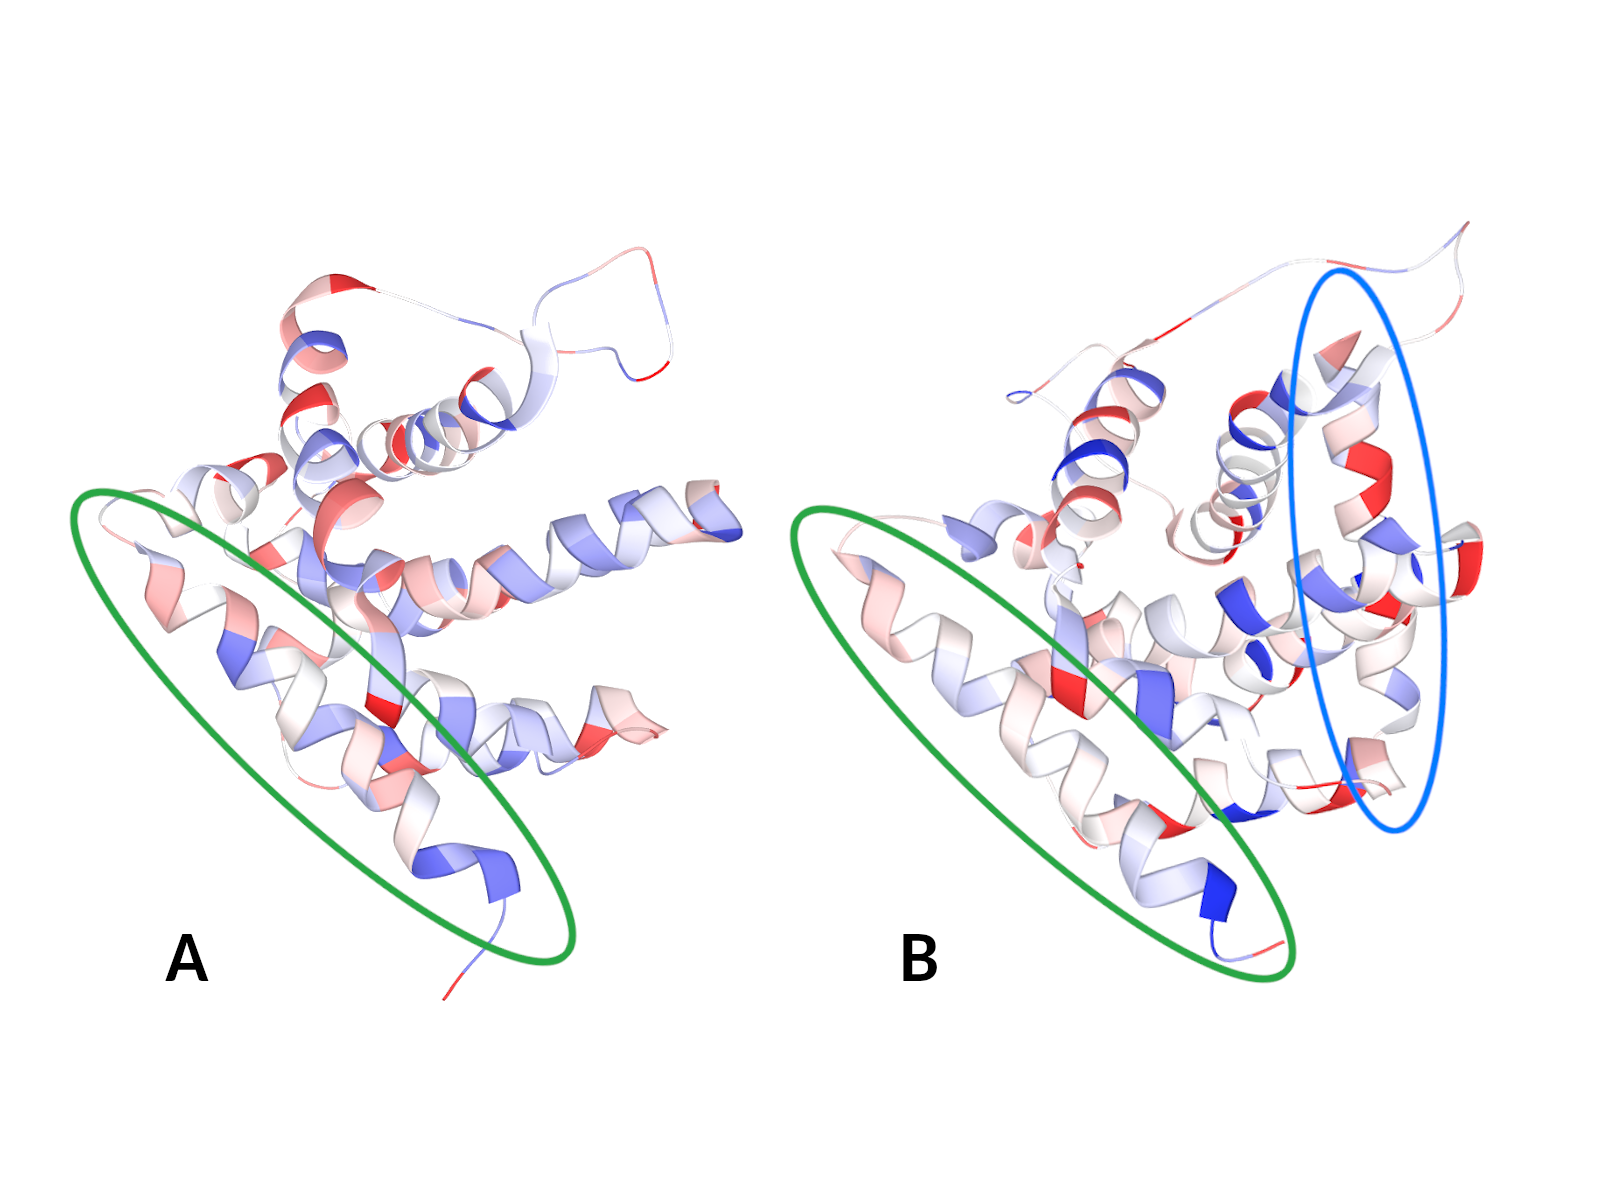
\includegraphics[width=.9\linewidth]{figure3.png}

\caption{A) Inactive BAX (PDB ID \href{https://www.ebi.ac.uk/pdbe/entry/pdb/1f16}{1f16}). B) Activated BAX (PDB ID \href{https://www.ebi.ac.uk/pdbe/entry/pdb/2k7w}{2k7w}). An activator is marked by a blue oval, C domain is marked by a green oval. C domain of activated BAX is depolarized -- has mainly white or whitish colour. This depolarization causes that C domain can be released and penetrate the mitochondrial membrane and start the apoptosis.}
\end{figure}

\end{document}